\section{Ohua}
\label{sec:back_ohua}

\begin{figure}[H]
    \centering
    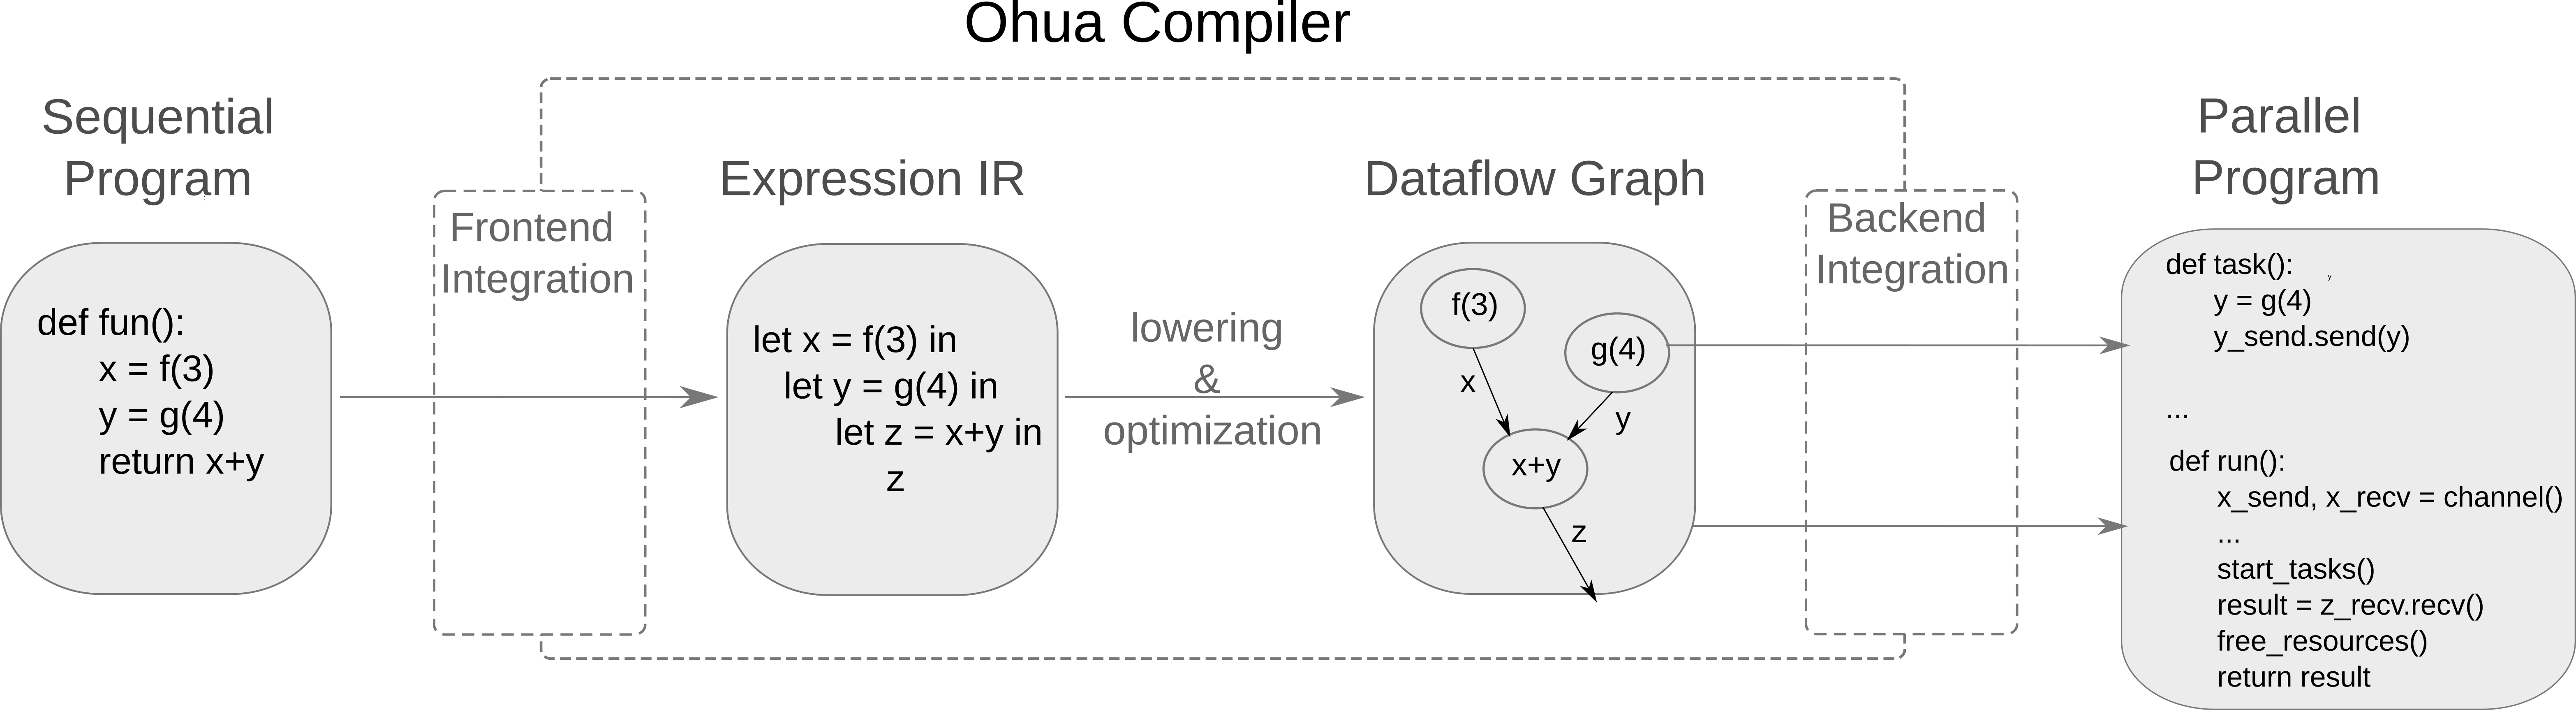
\includegraphics[scale= 0.36]{figures/ohua_fine_with_channels.png}
    \caption{Structural overview of Ohua and the code transformations}
    \label{fig:ohua_fine}
\end{figure}

\todo[inline]{Describe:}
\begin{enumerate}
    \item principle
    \item intermediate languages
    \item components/tasks of integrations
    \item assumptions of the programming model a) in the frontend b) in the backend (cooperative tasks, ordered messages, blocking receive etc.) 
\end{enumerate}

\subsection{Design and Principle}
\subsection{Programming Model/Frontend}
\subsubsection{Programming Model -- Expectations and Implications of program structure}
\begin{itemize}
    \item There are 3 kinds of functions:
    \begin{itemize}
        \item Algorithms: To make a clear distinction between functions in the compile scope and imported functions we term the former ones 'algorithms'. This distinction is important as we have different assumptions and processing of those two categories.
        \item pure functions
        \item stateful functions (i.e. methods)
    \end{itemize}
    \item Function arguments: Calls to functions or method outside the compile scope will end up in independent, concurrent tasks in the final program. Depending on the target 
    \item stateful computations are recognizable syntactically
    \item pure functions
    \begin{itemize}
        \item are considered side effect free
        \item in particular do not manipulate their input variables
        \item will be removed if the output is not used explicitly
    \end{itemize}
    \item Algorithms aka functions in the compile scope: 
    \begin{itemize}
        \item we currently only support functions, i.e. no methods but the reason might just be time to implement
        \item \question{do they 'finally' need to be pure? Can they take stateful arguments and alter them without returning? \means NO}
        \item 
    \end{itemize}
    \item[] Constructs inside algorithms:
    \item for-loops:
    \begin{itemize}
        \item indicate parallelizable loops
        \item to enable state threading, each state must be used linearly (only once) inside a loop
    \end{itemize}
    \item recursion/ while loops
    \begin{itemize}
        \item while loops are just another form of recursion 
        \item we currently only support tail recursion, with (only) recursive call in the if branch 
        \item \todo[inline]{Check recursion assumptions again when we managed while support}
        \item \question{linear state use assumed?}
        \item will lead to sequential code inside the recursion i.e. \todo[inline]{example} 
        \item IN case we don't make it and I need a reason: as while is just a (more restricted? Why?) form of recursion
        there is not too much scientific value in implementing it in our Ohua Prototype
        \item \todo[inline]{Sebastian: "Wir führen mit 'while' state threading für recursion ein". Was genau bedeutet das? Warum macht recursion das bislang nicht? Hierzu test mit stateful call als condition.}
        \item Note: The condition function of recursion/while is packaged in a node that returns a) a state if the condition was a stateful call and b) a tuple containing the boolean resulting from evaluation as often as it is needed downstream 
        \item arguments to recursive functions must be local variables. This means  
    \end{itemize}
    \item General Note: The allowed CFGs for input code are not freely composable, i.e. one can not simply put one valid CFG  into/around another to build a bigger one. This  goes beyond function borders as functions are inlined. \todo[inline]{Give example code. If possible list restrictions and give explanation at least concerning the nature of restriction as a) immanent feature of the IR/Programming Model or b) Current lack of implementation}
\end{itemize}

Aus ConDRust:
\todo[inline]{Check against description of current Rust subset}
\begin{itemize}
    \item supported terms are: variables, abstractions (closures), applications term(term) (Note: currying in the intermediate representation allows to convert closures with any number of arguments to one-argument-calls), mutable and immutable bindings, for-loops and tail-recursion(with part. restrictions)
    \item supported subset of rust (thereby general supported FR Language) is imperative \means allows mutable variables \means language syntax can express named memory locations (i.e. mapping from labels to memory locations) AND language evaluation semantics relates evaluation of terms to state of memory.
    \item values are: store/memory locations, actual Rust values (so far only some literals are directly supported, anything else has to be wrapped as a function return) and abstractions \question{How can abstractions be terms and values at the same time, when terms do not include values?}
    \item Types: To construct certain control nodes the presence of boolean, integer, tuple and list type (the later with constructors for empty list and prepend to linked list (a:as)) is expected. Apart from that general types, mutable  general types and references are supported
    \item  \question{The ConDRust paper says 'ConDRust's programming mode does not support references because ...' on the other hand types can be \rust{Ref<T>} and there is no restriction in the defined subset for usage of references a function argument or return or as type of pattern biding?}
    \item Stateless Calls: No side effects
    \item Stateful Calls: Side effects only on the calling state \rust{state1.do(state2, something)} \means no side effect on \rust{state2} or \rust{something} 
    \item \question{ConDRust: "We further restrict control
flow to loops and tail recursion leaving out other forms such as conditionals that play only a minor 
role in the parallel execution of a program." \means Generall wird if-else doch unterstützt und wie implementiert man eine Recusion ohne if? }
\item for-loops: bound or unbound, unbound-loops are internally represented as tail-recursions \question{Does this mean we can transform for-loops to tail recursion and if so, why can't we do the same thing with while ?} 
\item Rules for variable usage: 
\begin{enumerate}
    \item Variables can either be used as a State (calling stateful functions inside the compile scope) XOR used as an Argument to a function call. 
    \item If it is used as an Argument it may only be used once
    \item If it is used as a State it can be used more than once, except inside loops 
\end{enumerate}
\item Since the compiler can only check compliance with these rules on the basis of the syntax of the input program, the programmer can decide for himself whether, for example, duplication of data is really necessary if a variable is to be used twice. For example:\todo[inline]{Example for \rust{let c1, c2 = really_copy(c)} vs. \rust{let c1, c2 = just_refs_to(c)}} 
\end{itemize}

\subsection{Compiler Transformations}
\todo[inline]{not sure if this is an extra section, and if it should go between frontend and backend or after them as 'connector'}
Transformation roughly 
\begin{itemize}
    \item applicative normal form, SSA form \means explain
    \item transformation of stateful functions to state threads (basically \rust{let maybeResult = state.do()} becomes \rust{let (maybeResult, state) = state.do()}) making the state the output and input of it's stateful call, this makes sense even in the imperative representation as the actual name is overwritten in the downstream scope. It has also the effect of eliminating the need for a common storage among function calls.
    \todo[inline]{citations  [Ertel et al. 2019; Launchbury
and Peyton Jones 1994; Wadler 1992].}
\end{itemize}

\subsubsection{Backend Language/Process Abstractions}
A major advantage of compiling with Ohua is, that the generated dataflow-based language is deterministic. That is, a correct, deterministic, sequential program becomes a correct, deterministic, concurrent program by compilation. 
The essential syntactic elements and their semantics are already formally described in \todo[inline]{Can't cite STM paper while unpublished :-(}. In particular, these include the edges and nodes of the dataflow graph. An informal proof of the determinism of the resulting language is also given. 
Formal verification of this language is currently pending. Nevertheless, we can already clearly describe the assumptions concerning the realization of nodes, i.e. independent computational processes, and edges, i.e. communication channels between nodes.
Specifically, we assume for the implementation of nodes that:
\begin{enumerate}
    \item Nodes do not share memory (they may, but we don't assume them to do and Ohua will not make them do so)
    \item There can be more nodes than the run time is capable of running concurrently and there is no explicit scheduling. Therefore we assume cooperative multitasking i.e. nodes waiting for input will free computation resources for other nodes.
    \item \todo[inline]{Verify assumption} The run time instantiating the nodes is capable of ending them and freeing resources.
\end{enumerate}

Since it is a data flow language, the execution of the programs is controlled by the data flow. This results in the following assumptions for the implementation of the edges/data channels. 
\todo[inline]{Es ist (offensichtlich) exakt das Selbe wie im Grossen Beleg \means umformulieren aus formalen Gr\"unden n\"otig, inhaltlich sinnlos}
\begin{itemize}
    \item[i)] all data are transferred in order
    \item[ii)] there is no implicit use of default arguments (default arguments are in general possible, but there has to be an explicit signal for every computation in a node and every parameter it uses, that this parameter is 'None' and should be replaced by the default value for this particular execution round/loop)
    \item[iii)] receiving is blocking (this closely relates to ii) as such that there must not be a calculation or result passed on while it is not clear whether a term of that calculation just has not arrived at the moment of calculation) 
\end{itemize}


    
\subsection{Existing Rust Integration}
\label{subsec:RustIntegration}
Currently supported (working) subset
\begin{table}[H]
    \resizebox{\columnwidth}{!}{%
    \begin{tabular}{l c l l}
        \multicolumn{4}{l}{\emph{Block of Statements:}}\\
        $block$ & $::=$ & \textbf{\{}$s;~\ldots ;~s $\textbf{\}} & statements \\
        \multicolumn{4}{l}{\emph{Statements:} }\\
        $s$ & $::=$ & $ e $ & statement returning a value\\
        & $|$ & $ e $\textbf{;} & statement not returning a value\\
        & $|$ & \textbf{let} $pat$ \textbf{=} $e$ & local definition\\ 
        
        \multicolumn{4}{l}{\emph{Expressions:}}\\
        $e$ & $::=$ & $x$ & variable bindings \\
        & $|$ & $\textbf{1},\textbf{2},\textbf{3}, \ldots \ |\ \textbf{true}\ |\ \textbf{false}\ $  & literals \\
        & $|$ & $e$ \textbf{(}$e, \ldots , e$\textbf{)} & function calls \\
        & $|$ & $e$ $callRef$ \textbf{(}$e, \ldots , e$\textbf{)} & method calls \\
        & $|$ & $\textbf{(} e,~\ldots ,~e \textbf{)}\ $ & tuples\\
        & $|$ & $e\ +\ e\ |\ e\ -\ e \ |\ e\ > \ e\ |\ e\ == \ e\ |\ \ldots $ & binary operations \\
        & $|$ & $ -e\ |\ !e\ |\ *e\ $ & unary operations\\
        & $|$ &\textbf{if} $e$ $block$ \textbf{else} $e$& conditional with optional else branch \\
        % & $|$ & \textbf{while} $\ e$  $block$ & \\ % actually while loops are not supported at all
        & $|$ & \textbf{for} $pat$ \textbf{in} $e$ $block$ & \\ 
        & $|$ & \textbf{move} $\textbf{| } arg,~\ldots ,~arg \textbf{ |}\ e$ & closure\\
        &$|$& $block$ & block expression, i.e. block returning a value\\
        \multicolumn{4}{l}{\emph{Call References:}}\\
        $callRef $ & $::=$ & $ z\textbf{.}y\textbf{.}x$ $[gernericArg]$  & namespaced binding  \\
        \multicolumn{4}{l}{\emph{Patterns:}}\\
        $pat$ & $::=$ & $x\ |\ (x,~\ldots ,~x)|\ \_ $ & bindings, tuples or wild cards \\
    \end{tabular}%
    }
    \caption{Subset of Rust grammar, that is accepted by the integration frontend}
    \label{tab:FESubset}
\end{table}


\section{smolTCP}
smolTCP~\cite{smolTCP} is a Rust-based open-source implementation of a TCP/IP stack. It runs entirely as a user space application and without heap allocation, making it amenable be used in microkernels as M$^3$\cite{Asmussen:M3v} and embedded systems such as ARTIQ (e.g. \cite{lam2021combining}). Redox\cite{redoxwebsite} a microkernel operating system implemented in Rust uses smoltcp as network stack implementation.

\begin{figure}[H]
    \centering
    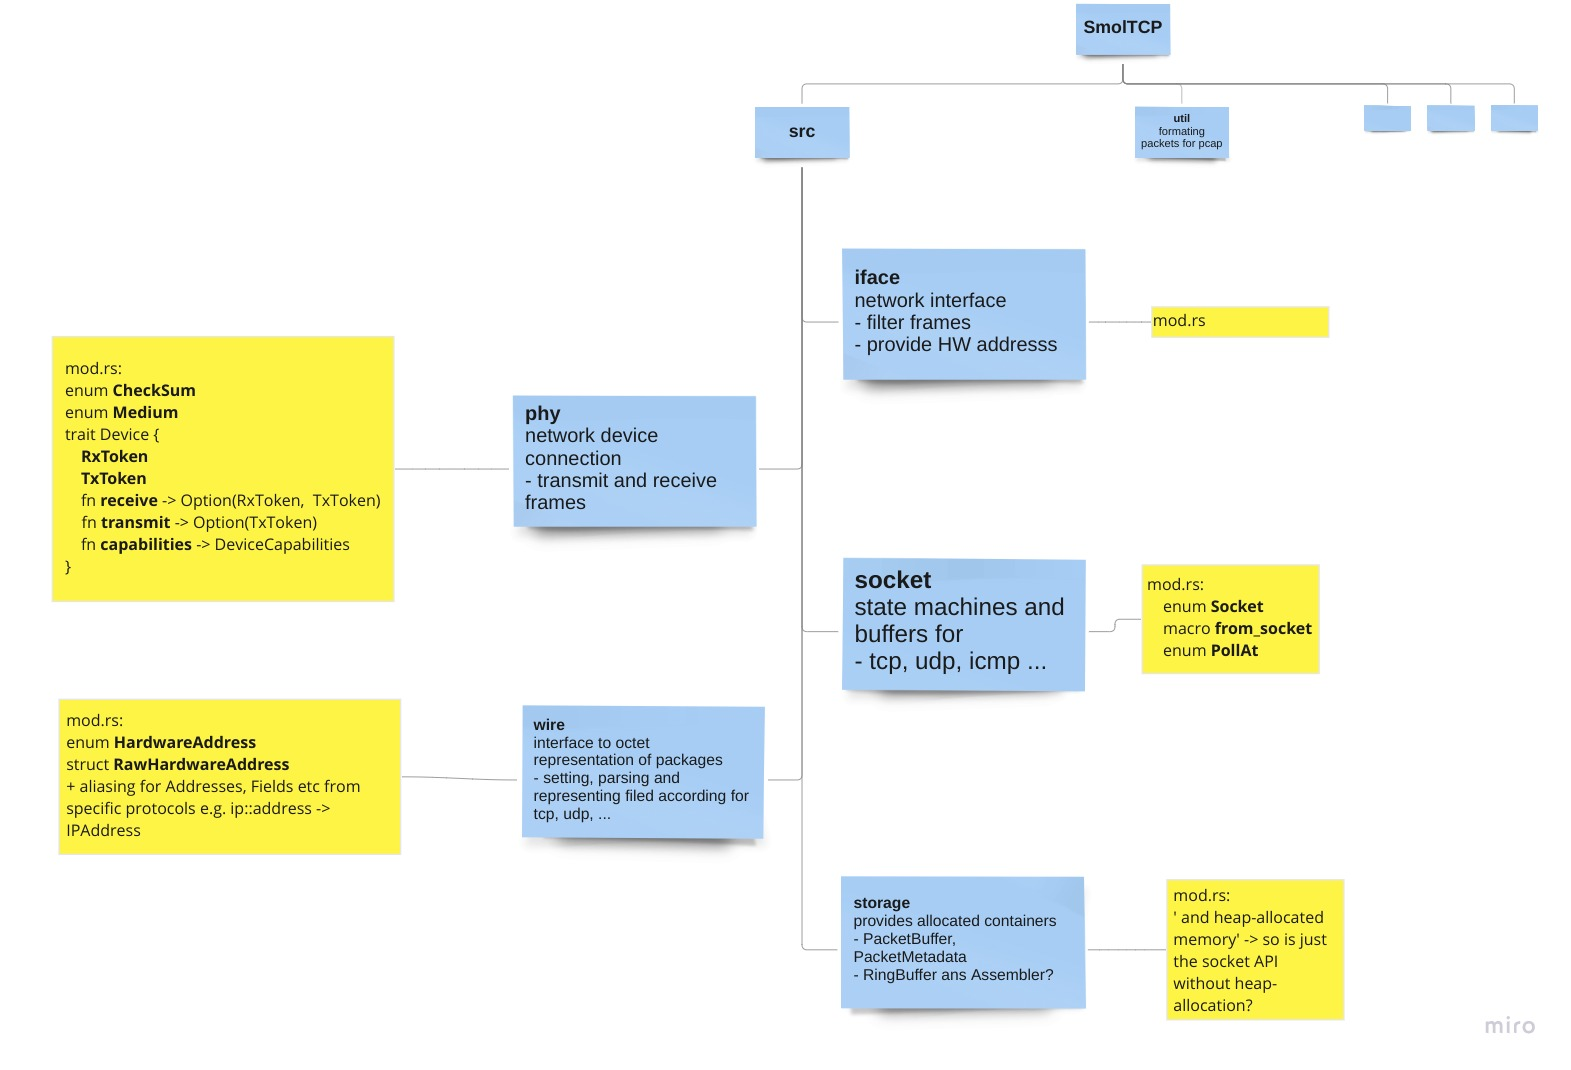
\includegraphics[scale= 0.33]{figures/SmolTCP - Overview.jpg}
    \caption{Structural overview of smoltcp. Currently the TCP/IP Stack, basically implemented in the \textbf{socket} and iface modules \textbf{interact} with the 'physical' network interfacing implemented in the \textbf{phy} and \textbf{wire} modules via simple function calls using references to shared objects. This only works in Monolithic and Unikernels, where they share the same adress space}
    \label{fig:smoltcp_components}
\end{figure}




\section{Microkernels/Unikernels}

\textbf{Unikernel}
General purpose operating system have to provide a broad range of functionality to connect application layer to hardware layer. This is includes user interfaces (graphics), networking, security, device drivers and most obviously the functionality required for program execution and memory management, which may also include virtualization mechanisms for programming languages as Java and Python. For microservices however large parts of those general purpose systems are not required. For example, a microservice that merely answers simple requests to a key-value store only needs the functionality of the network stack and the file system. Libraries and system functions for additional user or device interfaces only unnecessarily increase the complexity, memory consumption and attack surface of the service.\\

The concept of Unikernels accounts for this problem \cite{madhavapeddy2014unikernels}. Its general principle is, to compile a kernel specifically for a given application, such that it only provides required functionality. 
\todo[inline]{What kind of organization is unikernel.org? \cite{unikernelorg}}
Examples of this are CubicleOS~\cite{sartakov2021cubicleos}, FlexOS~\cite{lefeuvre2021flexos} and M$^3$x~\cite{Asmussen:M3x}, M$^3$v~\cite{Asmussen:M3v}.
\todo[inline]{read \cite{madhavapeddy2014unikernels},CubicleOS~\cite{sartakov2021cubicleos}, FlexOS~\cite{lefeuvre2021flexos} and M$^3$x~\cite{Asmussen:M3x}, M$^3$v~\cite{Asmussen:M3v} \means how are the kernels compiled, what's there scope? }

\textbf{Unikernels\cite{madhavapeddy2014unikernels} $\blacktriangleright$} single purpose, specialized OS kernels; written in a high-level language; act as individual, potentially distributed components of a full application/software \means the hypervisor controls eg. unikernels for file system, network stack and user process instead of VMs running all those together \means full scaling control is shifted to the hypervisor level, only required resources are scaled

\textbf{Library Operating Systems}: actually provide the basis for compiling Unikernels; library operating systems provide functionalities of monolithic kernels as independent library implementations e.g. device drivers for physical NICs are implemented in libraries that can be combined with potentially different implementations of the TCP/IP stack. 'MirageOS' is a library operating system.

\textbf{Microkernel$\blacktriangleright$} The central motivation for microkernels, is the reduction of privileged, low-level code executing in kernel mode. Based on the insight, that large code bases of monolithic kernels com e at the costs of large potential for bugs in privileged, low-level (and therefore hard to check) code concepts to minimize kernels and therefore attack surface date back to the 70$^th$. 
\todo[inline]{collect citations: Brinch Hansen 1970; Wulf et al. 1974; Accetta et al. 1986; Liedtke 1993; Shapiro et al. 1996; Hohmuth et al. 2004, separation kernels  Rushby 1981; Information Assurance Directorate 2007, the MILS approach [Alves-Foss et al. 2006], isolation kernels [Whitaker et al. 2002],the use of type-safe languages for all code except some ''dirty'' core [Bershad et al.
1995; Fahndrich et al. 2006]}
\means microkernels follow a \textit{minimality principle} formulated by Liedtke~\cite{jochen1995mu} as ''More precisely, a concept is tolerated inside the $\mu$-kernel only if moving it outside the kernel, i.e. permitting competing implementations, would prevent the
implementation of the system's required functionality.''. This basically limits the essential components of kernel to memory management (i.e. providing access and access control to address spaces), CPU allocation (i.e. providing access to the CPU in any form of process or thread abstraction and scheduling) and inter-process communication (IPC).\means system services as I/O, device drivers, networking and others run as userland processes although there might be further distinctions from actual user processes (e.g. in MINIX 3 device drivers still have direct HW access and operating system functionality is run by so called \textbf{server}, a term that commonly comes up for those 'outsourced' basic functionality) \means this design comes with an inherent performance penalty because, instead of 'contacting' kernel space once and waiting for the result, the request of one client/user application will be forwarded by the kernel via process communication e.g. to a driver process, who again answers via IPC indirected through the kernel i.e. 4 context switches instead of 2 as in the monolith, further communication among system services is just function calls in monoliths while it's again IPC+4 context switches in microkernels. 

\begin{figure}[H]
    \centering
    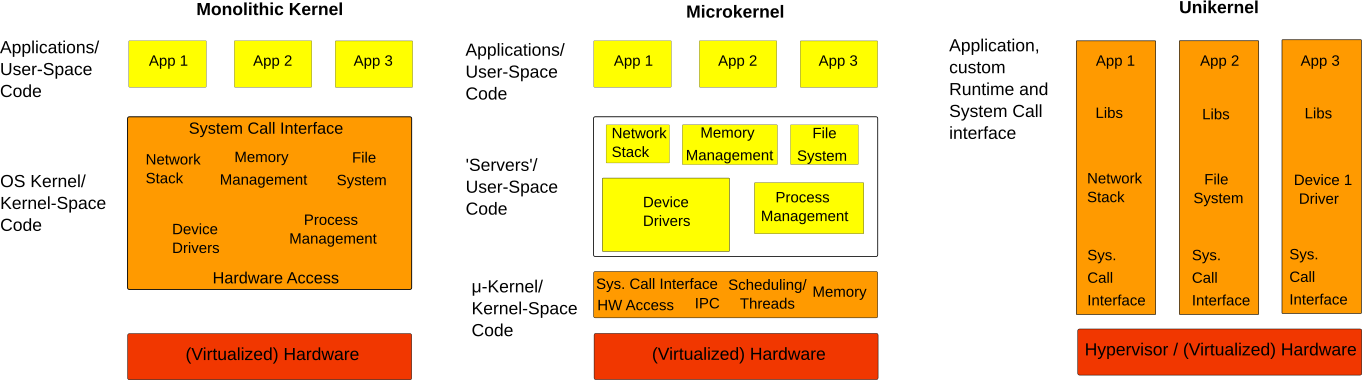
\includegraphics[scale= 0.36]{figures/kernels.png}
    \caption{Structural comparison of Monolithic, Micro- and Unikernels }
    \label{fig:kernels}
\end{figure}


\todo[inline]{Example Rust 4 Unikernel \cite{Rust4Unikernel}}
\todo[inline]{Formal Verification eg for L4 derivatives as motivation \cite{sL4Verf}}

Examples:
\begin{itemize}
    \item[$\mu$-kernel]: L4, Mach (first generation $\mu$-kernel), Minix, Singularity, NOVA
    \item[$\mu$-kernel OSs]: QNX (embedded systems\means phones, real time OSs \means cars, alive and kicking, unix-like; own microkernel named pronto?), MINIX 3 (embedded+education, dormant since 2017; POSIX comp., own open source $\mu$-kernel), lots of examples on the slide from 'Microkernel Construction'(Intro)
    \item[libOSs]: Unikraft~\cite{kuenzer2021unikraft}, IncludeOS~\cite{bratterud2015includeos}, Graphene~\cite{tsai2014Graphene}
    \item[unikernels]:
\end{itemize}

\section{Our target Backend $M^3$:}
\subsection{The Concept}
\begin{itemize}
    \item M$^3$ is a micro kernel concept/architecture for distributed and potentially heterogeneous architecture
    \item for example as embedded system in mobile devices
    \item it's based on a hardware-OS-co-design approach i.e. specialized HW components for special OS tasks (or the other way around) e.g. separate chips for broadband communication, signal processing (camera, GPS), maybe crypto per device.
    \item specialty of the HW design \means HW components 'tiles' are connected via Trusted Communication Units (TCUs)
    \item the actual (micro) kernel runs on one tile and is the only component privileged to establish communication among other tiles via the TCUs
\end{itemize}
detailed
\begin{itemize}
    \item system architecture to integrate heterogeneous 'compute units' 
    \item CU: computing units with pot. different ISAs e.g. general purpose CPUs, FPGAs, DSPs, fixed-function accelerators
    \item Operating system should let each CU: 
    \begin{itemize}
        \item work independently + isolated (in the security sense)
        \item switch context\means Kernel can schedule other tasks on a CU and swithc them for better HW utilization
        \item communicate directly to each other i.e. no central CPU
        \item access OS services like file system and network stack
    \end{itemize}
    \item How: 
    \begin{itemize}
        \item DTUs: data transfer units are a HW component M§ introduces as common interface at each CU, this allows coherent access to/from the OS
        \item OS Kernel runs on a dedicated CU, controlling the other services 'remotely' via their DTUs 
        \item Context switching means, switching from the execution of one program/ call to another 
        \item Activity: A running entity on a CU, for CPU generally a system thread
        \item Communication with suspended activities (A \means B, B is suspended): So called fast-path communication i.e. communication directly among two Activities without involving the kernel is default. Activities are not aware if their communication partner is currently running or suspended i.e. context was switched by kernel. The lazy approach taken by M3(x) means, the HW detects attempts to communicate with a not-running Activity and errors back to the sending activity. Upon such error, the sending activity A invokes the kernel to schedule B and asserts delivery of message. 
        \item Idle Notification: when activities idle they notify the kernel, which can then schedule another activity
        \item to efficiently schedule an application with many "heavily communicating" activities, a \textbf{Gang schedule} mechanism can be used  by defining the 'gang' of an activity at creation time (?). \means we might use this 
        \item Accelerators: There's two types of them considered 1) request processing accelerators (get a blob of data \means process \means return) 2) stream processing accelerators (get a file/source \means stream process data to a sink). There's ASM (Accelerator Support Module) for both \means not sure we'll need to know this
        \item OS Services - File Access: implemented as 'microservice-style servers', applications and accelerators are clients, access to files via \code{next_in} and \code{next_out} i.e. client (accelerator) requests input and output source, gets \code{next_in} and \code{next_out} and infos on the offset and can retrieve data from/write output to memory using this info without asking the server again. The server has no direct control what is read/written \means follow up requests are considered 'commits' on the previous sections being processed completely \means \textbf{Can/Do we keep that promise? Is it by design or does the software have to comply explicitly?}
    \end{itemize}
    \item Implementation: 
    \begin{itemize}
        \item kernel tile \means runs micro kernel, controls DTUs of 'everybody'
        \item user tiles \means run activities, send sys calls as messages to the kernel, by default they are disconnected from each other
        \item each activity has it's own address space and capabilities, capabilities can be shared via sys calls
        \item system services implemented as servers \means eg. m3fs file system similar to UNIX but grant direct access via DTU, pipe server establishing \textbf{ unidirectional, first-in-first-out communication channel} between activities
        \item context switches \means  placement/scheduling decision by kernel, state of suspended activity saved locally by special component on each user tile (remotely controlled time multiplexer (RCTMux), for general purpose CPUs they are just software), state of DTU (i.e. access rights and channels) stored by the kernel for security reasons, messages for suspended activities are redirected to and buffered by the kernel until rescheduling of the recipient
        \item addressing and forwarding messages: messages have sender and receiver IDs, if a DTU notices $receiverID != currentID$, it errors to $senderID$ so the sender can forward the message to the kernel instead
        \item messages have only-once semantic, data-access can/must be repeated during execution/upon failure
        \item the M3x standard library wraps the \code{next_in}, \code{next_out}, \code{commit} and \code{search} file server communication in a UNIX like API for file access 
        \item file system access for accelerators is implemented in HW, input and output stream (for streaming accelerators) consist of a message and a data channel each
    \end{itemize}
\end{itemize}
\means seems we have (according to design) loss-less communication in order and preemptive scheduling and tasks go idle upon receiving \means looks good concerning our assumptions. 
\todo[inline]{There are different platforms to simulate/host/run M3. Maybe describe them here or in the benchmark section.}

\subsection{The Rust API}
Any backend integration for Ohua needs to specify the implementation for two core primitives of Ohuas DFG language, namely an implementation for the nodes of the Data Flow Graph and an implementation for the edges i.e. the communication channels both following the assumptions of the programming model as described in Section~\ref{sec:back_ohua}. M3 provides a Rust integration to access its abstractions of processes and channels. We will now describe the main features of this API. \\
\todo[inline]{ Maybe extend this description later to really cover the basic features}

To run processes in M3, one first needs to instantiate at least one \rust{Tile}\todo[inline]{lookup struct}. Tiles are M3 abstraction of computing units. Processes running on tiles are called \rust{activity}\todo[inline]{lookup struct}. So we can choose to instantiate the nodes of the DFG as \rust{activity} on the same or different tiles
\todo[inline]{What have we chosen}. To pass initial data to an activity, the attribute \rust{activity.sink()} can be used to serialize data into the process memory. This data can be accessed from inside the activity code using \rust{activity.source()}. Serialization is done using \code{serde} \question]{couldn't find ... ask Nils again}
This is necessary e.g. when a parent process needs to pass some process state to a child process as each activity is spawned i.e. starts without inheriting anything from the parent. \question{Ask Nils: Activities are started as closures. So do we need that source-sink mechanism for imports, consts etc or only for runtime stuff from the main?}. As shown in Figure~\ref{fig:startingActivity} activities are created as closures just as normal threads in Rust. They also mimick the behaviour of normal Rust threads regarding their interfaces for starting them using \code{run}, terminating them using \todo[inline]{Insert terminate call}. They are terminated and their memory is cleaned automatically as soon as they go out of scope.\\ 

\todo[inline]{Figure showing Code for an activity}
\begin{figure}
    \centering
    \begin{minted}{rust}

// Code for starting activity goes here
    
    \end{minted}
    \caption{Creating and running a Rust activity on M3}
    \label{fig:startingActivity}
\end{figure}

Concerning process communication, M3 provides different mechanisms, mainly depending on the size of data to be transmitted. \todo[inline]{Check the other ones when Nils is back}. M3 manages communication among processes using capabilities. The capability to directly send to or receive from another process is implemented as \rust{Gate}s in the M3 Rust API. Gates are directed one-to-one connections, so there are send gates \rust{SGate} and receive gates \rust{RGate}. Receive gates are instantiated with a maximum message size and a maximum overall size of the message buffer to prevent memory overflows in limited environments. The absolute (system immanent) maximum message size is 2 kb. A selector, i.e. an ID of those gates must be delegated to the activities explicitly. Any connection among activities, even on the same tile has to be permitted by the kernel tile and registered at the DTUs of the tiles on which the activities run. This happens automatically for sending gates when the first message is send, but has to be done manually by calling \rust{activate} on the gate handle. \\
\todo[inline]{Check: "Mit dem Selektor muss ein neues Gate in der Activity instantiiert und gebunden werden"}

Sending messages is straight forward as known from most pipe like interfaces. Receiving is done in two steps. First a receive stream is requested using \rust{let stream = rgate.recv_msg()}. This is a blocking call, that will return upon available  messages arriving at the gate. The second step is calling \rust{let msg = stream.pop()} which is non blocking. This call can be done arbitrarily often on an existing stream but will fail if there are no more messages in the stream. Another special feature of the M3 gates is the forcing of a credit system. To prevent too many messages from being sent, the sender requires one credit for each message. To get the credit back after sending a message, the receiver must reply to the message using \rust{reply_vmsg!(/*arbitrary list of reply items*/)} and the sender must receive this reply. Per received reply, the sender will regain one sending credit. It is possible when creating the gates to specify a number of messages that may be sent before new credits are required. The mechanism is similar to the window size in TCP. However, in the end there must be a credit for each message and it is not possible to initialize a send gate e.g. with an arbitrary number of credits. So contrary to the existing integrations, we will have to implement a bidirectional mechanism of message receipt.\\

Finally a limitation of the current M3 API is that the standard library is not supported. There is a separate implementation of \rust{std} with essential functions but partly different function signatures. For smoltcp itself this limitation is not relevant, since it is written without using the standard library. In contrast, the libc API is a necessary part of smoltcp and is supported by M3. 



\section{Rust}
\todo[inline]{Not sure if I'll need this but collect some infos e.g. closures and the heaplessness of smoltpc at least so I know what the implications are}
\textbf{Closures}: Closures are used in smotcp quite a lot so its important to understand how this influences state sharing and control flow in the original architecture.
\begin{itemize}
    \item if not explicitly annotated, the closure will derive if captured objects are mut/immut borrowed or moved 
\end{itemize}
\begin{minted}{rust}
let obj1 = OBJ1::new();
let closure1 = |arg| {let x =obj1.do_stuff(arg);
                      x*2}
// closure1 is moved to use_closure, 
// while obj2 gets a mutable reference to obj1
obj2.use_closure(closure1);
\end{minted}

Features of Rust that might become relevant for implementation
\begin{itemize}
    \item Type Inference: Rusts type inference is based on standard Hindley-Milner (HM) type inference algorithm\footnote{Full description can be found in \href{https://rustc-dev-guide.rust-lang.org/about-this-guide.html}{the Guide to Rustc Development}}. To resolve trait bounds a Unification algorithm similar to the algorithm used in Prolog to solve logical constraints\footnote{The Trait Bound Unification is implemented in the \href{https://rust-lang.github.io/chalk/book/}{Chalk} library}.
    \todo[inline]{If needed and time allows check (reasons for) limitations and give details on extensions}
    \item Generic Types: To allow the use of generic types with basically no runtime overhead, Rust uses so called \textit{monomorphization} at compile time. This process infers concrete typing for any use of generically typed elements, like functions, structs or enums. The concretely typed instances of elements are then inlined to the existing code. It is in fact one of the last steps on a Rust IR before the code is lowered to LLVM IR and passed to LLVM for code generation and enables LLVM to infer some lower level optimizations (city rustc guide again? ).
    \item Serialization: There is a crate \href{https://doc.rust-lang.org/nightly/nightly-rustc/rustc_serialize/index.html}{serialize}, that as described in the 
\end{itemize}